% !TEX root = ../notes_unsupervisedlearning.tex
% Chapter 14: World Models and Vision-Language-Action Models
%%%%%%%%%%%%%%%%%%%%%%%%%%%%%%%%%%%%%%%%%%%%%%%%%%%%%%%%%%%%%%%%%%%%%%

\chapter{World Models and Vision-Language-Action Models}\index{World Models}\index{VLA}\index{Embodied AI}
\newthought{Simulate, imagine, then act in the real world.}

%═══════════════════════════════════════════════════════════════════════
% BLOCK 1: INTRODUCTION
%═══════════════════════════════════════════════════════════════════════

\section{The Why}

\marginnote{Humans imagine consequences before acting; can machines learn to do the same?}

Model-free RL learns from experience, but it is sample-inefficient, requiring millions of environment interactions; unsafe, because learning by trial-and-error can be dangerous; and non-transferable, because the agent must relearn for each new task.

\newthought{Model-based RL}\index{model-based RL} learns a model of the world, enabling planning by simulating actions before taking them, imagination by generating synthetic experience for training, and sample efficiency by learning from fewer real interactions.

\newthought{Vision-Language-Action models}\index{VLA} represent the frontier: systems that see, understand language, and act in the physical world.

\newthought{In order to move from trial-and-error to planning in imagination} we have good reason to find ways to,
\begin{itemize}
    \item learn dynamics models that predict future states and rewards from current states and actions, enabling mental simulation.
    \item drive exploration via intrinsic motivation so that the agent seeks novel states even when extrinsic rewards are sparse.
    \item unify vision, language, and action in a single architecture so that web-scale knowledge transfers to robotic control.
\end{itemize}

\subsection{Hands On Experience}

\begin{marginfigure}
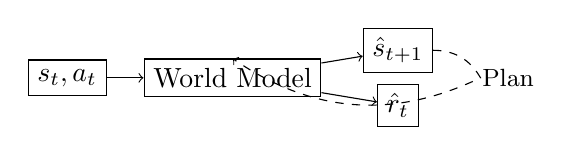
\begin{tikzpicture}[scale=0.7]
    % World model
    \node[draw, rectangle, minimum width=2cm] (wm) at (0,0) {World Model};
    % Input
    \node[draw, rectangle] (s) at (-3,0) {$s_t, a_t$};
    % Output
    \node[draw, rectangle] (sp) at (3,0.5) {$\hat{s}_{t+1}$};
    \node[draw, rectangle] (r) at (3,-0.5) {$\hat{r}_t$};

    \draw[->] (s) -- (wm);
    \draw[->] (wm) -- (sp);
    \draw[->] (wm) -- (r);

    % Planning loop
    \draw[->, dashed] (sp.east) to[bend left] (4.5,0) to[bend left] (wm.north);
    \node at (5,0) {\small Plan};
\end{tikzpicture}
\caption{World model predicts next state and reward, enabling mental simulation.}
\label{fig:world_model_intro}
\end{marginfigure}

Imagine you are learning to play a video game:
\begin{enumerate}
    \item After playing briefly, you can imagine what happens if you jump
    \item You simulate different strategies in your head
    \item You execute the best plan in the real game
\end{enumerate}

This is planning with a learned model: act in imagination, then act in reality.

\newthought{The Learning Objectives} of this lecture:
\begin{itemize}
    \item Explain model-based RL, describe world model architectures such as Dreamer, and identify how model errors compound over long planning horizons.
    \item Implement curiosity-driven exploration and distinguish intrinsic from extrinsic reward signals.
    \item Describe VLA architectures and articulate how web-scale vision-language knowledge transfers to robotic control.
\end{itemize}

%═══════════════════════════════════════════════════════════════════════
% BLOCK 2: MAIN THEORY
%═══════════════════════════════════════════════════════════════════════

\newpage
\section{Model-Based Reinforcement Learning}\index{model-based RL}

\marginnote{Learn a model, then plan with it.}

\subsection{The Dynamics Model}

\newthought{Learn $f_\theta$} to predict:
\begin{equation}
    \hat{s}_{t+1}, \hat{r}_t = f_\theta(s_t, a_t)
\end{equation}

Training is supervised learning on collected transitions $(s, a, r, s')$.

\subsection{Planning with the Model}

\newthought{Model Predictive Control}\index{MPC}:
\begin{enumerate}
    \item At state $s$, simulate many action sequences
    \item Evaluate cumulative reward for each
    \item Execute first action of best sequence
    \item Repeat at next state
\end{enumerate}

\begin{algorithm}[H]
\caption{MPC with Learned Model}
\begin{algorithmic}[1]
\Require Current state $s$, model $f_\theta$, horizon $H$, samples $N$
\For{$i = 1$ to $N$}
    \State Sample action sequence $a_1^i, \ldots, a_H^i$
    \State $\hat{s} \gets s$
    \State $R_i \gets 0$
    \For{$t = 1$ to $H$}
        \State $\hat{s}, \hat{r} \gets f_\theta(\hat{s}, a_t^i)$
        \State $R_i \gets R_i + \gamma^{t-1} \hat{r}$
    \EndFor
\EndFor
\State \Return $a_1^{i^*}$ where $i^* = \arg\max_i R_i$
\end{algorithmic}
\end{algorithm}

\subsection{Model Error and Compounding}\index{model error}

\marginnote{Model errors compound over long horizons.}

\newthought{Small prediction errors accumulate:}
\begin{equation}
    \text{error at step } H \approx H \cdot \epsilon_{\text{single-step}}
\end{equation}

Mitigation strategies include short planning horizons, ensemble models, and frequent re-planning.


\section{World Models}\index{world model}

\marginnote{World models: compress observations into latent space, predict in latent space.}

\subsection{Ha and Schmidhuber (2018)}\index{Ha-Schmidhuber world model}

\newthought{The architecture} has three components~\cite{Ha2018WorldModels}:
\begin{enumerate}
    \item Vision (V): a VAE encodes observations to latent $z$
    \item Memory (M): an RNN predicts future latents
    \item Controller (C): a simple policy on $(z, h)$
\end{enumerate}

\begin{figure}
\centering
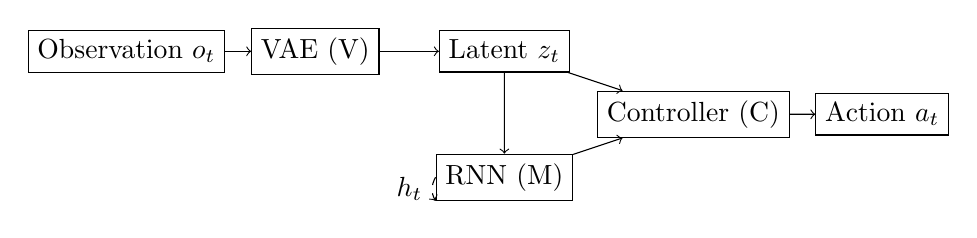
\begin{tikzpicture}[scale=0.8]
    \node[draw, rectangle] (obs) at (0,0) {Observation $o_t$};
    \node[draw, rectangle] (vae) at (3,0) {VAE (V)};
    \node[draw, rectangle] (z) at (6,0) {Latent $z_t$};
    \node[draw, rectangle] (rnn) at (6,-2) {RNN (M)};
    \node[draw, rectangle] (ctrl) at (9,-1) {Controller (C)};
    \node[draw, rectangle] (act) at (12,-1) {Action $a_t$};

    \draw[->] (obs) -- (vae);
    \draw[->] (vae) -- (z);
    \draw[->] (z) -- (rnn);
    \draw[->] (z) -- (ctrl);
    \draw[->] (rnn) -- (ctrl);
    \draw[->] (ctrl) -- (act);
    \draw[->, dashed] (rnn.west) to[bend right] node[left] {$h_t$} (rnn.south west);
\end{tikzpicture}
\caption{World Models architecture: V compresses, M predicts, C acts.}
\label{fig:world_models}
\end{figure}

\newthought{The key insight:} train V and M on real experience, then train C entirely in imagination.

\subsection{Dreamer}\index{Dreamer}

\marginnote{\newthought{Dreamer.} State-of-the-art latent world model~\cite{Hafner2020Dreamer}.}

\newthought{Dreamer learns} four components:
\begin{itemize}
    \item Representation model: $p(s_t | s_{t-1}, a_{t-1}, o_t)$
    \item Transition model: $p(s_t | s_{t-1}, a_{t-1})$
    \item Reward model: $p(r_t | s_t)$
    \item Decoder: $p(o_t | s_t)$
\end{itemize}

\newthought{Actor-critic in imagination:} imagine trajectories using the transition model, estimate values using imagined rewards, and update the policy to maximise imagined return.


\section{Exploration and Curiosity}\index{curiosity}\index{intrinsic motivation}

\marginnote{Sparse rewards require intrinsic motivation to explore.}

\subsection{Intrinsic Motivation}

\newthought{Add intrinsic reward} for visiting novel states:
\begin{equation}
    r_{\text{total}} = r_{\text{extrinsic}} + \beta \cdot r_{\text{intrinsic}}
\end{equation}

\subsection{Curiosity-Driven Exploration}\index{ICM}

\newthought{The Intrinsic Curiosity Module}~\cite{Pathak2017Curiosity}:
\begin{equation}
    r_{\text{intrinsic}} = \|f_\theta(s_t, a_t) - s_{t+1}\|^2
\end{equation}

High prediction error indicates a novel state, which yields high reward.

\newthought{The noisy TV problem:} random noise is unpredictable but not interesting. The agent wastes time on inherently stochastic signals.

\subsection{Random Network Distillation}\index{RND}

\newthought{RND}~\cite{Burda2019RND} uses a fixed random network $f$ that maps states to features and a learnable network $\hat{f}$ that tries to match $f$. The intrinsic reward is $\|f(s) - \hat{f}(s)\|^2$. Novel states are hard to match because $\hat{f}$ has not seen them.


\section{Vision-Language Models for Robotics}\index{vision-language model}

\marginnote{VLMs: understand images and text together.}

\subsection{From CLIP to Robotics}

\newthought{Foundation models provide} visual understanding to recognise objects, scenes, and attributes; language grounding to connect words to visual concepts; and common sense as implicit knowledge about the world.

\newthought{The key question:} how to connect perception and language to action?

\subsection{PaLM-E: Embodied Multimodal Reasoning}\index{PaLM-E}

\newthought{PaLM-E} injects visual tokens into a large language model~\cite{Driess2023PaLME}. The model can reason about images and plan actions, outputting natural language plans or action tokens.


\section{Vision-Language-Action Models}\index{VLA}

\marginnote{VLAs: the next step in embodied AI.}

\subsection{RT-1: Robotics Transformer}\index{RT-1}

\newthought{RT-1} takes an image and a language instruction as input and outputs discretised robot actions~\cite{Brohan2022RT1}. It was trained on 130k real robot demonstrations.

\begin{figure}
\centering
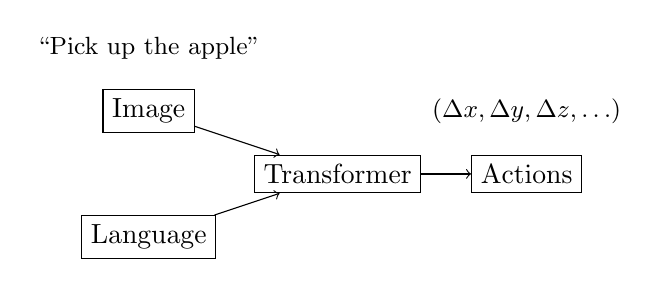
\begin{tikzpicture}[scale=0.8]
    \node[draw, rectangle] (img) at (0,1) {Image};
    \node[draw, rectangle] (lang) at (0,-1) {Language};
    \node[draw, rectangle, minimum width=2cm] (enc) at (3,0) {Transformer};
    \node[draw, rectangle] (act) at (6,0) {Actions};

    \draw[->] (img) -- (enc);
    \draw[->] (lang) -- (enc);
    \draw[->] (enc) -- (act);

    \node at (0,2) {\small ``Pick up the apple''};
    \node at (6,1) {\small $(\Delta x, \Delta y, \Delta z, \ldots)$};
\end{tikzpicture}
\caption{VLA architecture: image + language $\to$ transformer $\to$ robot actions.}
\label{fig:vla}
\end{figure}

\subsection{RT-2: VLM as Robot Policy}\index{RT-2}

\newthought{RT-2} fine-tunes a vision-language model for action prediction~\cite{Brohan2023RT2}. Actions are encoded as text tokens, and the model inherits the VLM's reasoning and generalisation.

\subsection{OpenVLA: Open-Source VLA}\index{OpenVLA}

\newthought{OpenVLA} is a 7B parameter model trained on the Open X-Embodiment dataset~\cite{Kim2024OpenVLA}. It supports multiple robot embodiments and provides open weights for research.


\section{Towards Embodied AI}\index{embodied AI}

\marginnote{The ultimate test of intelligence: acting in the physical world.}

\subsection{Sim-to-Real Transfer}\index{sim-to-real}

\newthought{Train in simulation, deploy on a real robot:} domain randomisation varies simulation parameters, system identification matches simulation to reality, and real-world fine-tuning adapts with real data.

\subsection{Open Challenges}

\newthought{Key challenges remain:} safety, because robots can cause harm; generalisation across environments; data scarcity, because robot data is expensive to collect; and multimodality, because touch, sound, and proprioception remain underexplored.


\section{Course Synthesis}

\marginnote{The full arc: from clustering to embodied agents.}

\begin{figure}
\centering
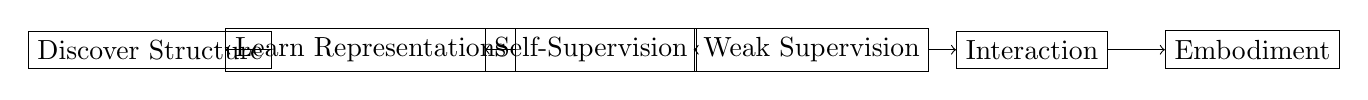
\begin{tikzpicture}[node distance=0.8cm, scale=0.7]
    \node[draw, rectangle] (struct) at (0,0) {Discover Structure};
    \node[draw, rectangle, right of=struct, xshift=2cm] (repr) {Learn Representations};
    \node[draw, rectangle, right of=repr, xshift=2cm] (self) {Self-Supervision};
    \node[draw, rectangle, right of=self, xshift=2cm] (weak) {Weak Supervision};
    \node[draw, rectangle, right of=weak, xshift=2cm] (interact) {Interaction};
    \node[draw, rectangle, right of=interact, xshift=2cm] (embody) {Embodiment};

    \draw[->] (struct) -- (repr);
    \draw[->] (repr) -- (self);
    \draw[->] (self) -- (weak);
    \draw[->] (weak) -- (interact);
    \draw[->] (interact) -- (embody);
\end{tikzpicture}
\caption{The course arc: from structure to embodied intelligence.}
\label{fig:course_arc}
\end{figure}


%═══════════════════════════════════════════════════════════════════════
% BLOCK 3: STUDENT ACTIVATION
%═══════════════════════════════════════════════════════════════════════

\newpage
\section{Examples \& Exercises}

\subsection{Exercise 1: World Model Design}

You want to learn a world model for a driving simulator. Design the architecture:
\begin{enumerate}
    \item What is the input?
    \item What should it predict?
    \item How would you train it?
\end{enumerate}

\subsection{Exercise 2: Curiosity Trade-offs}

A robot explores a room. The TV shows random static. Why might curiosity-driven exploration spend too much time watching the TV?

\subsection{Exercise 3: VLA Advantages}

Why might a VLA trained on internet data generalise better than a robot-only model?


\section{Self-Reflection and Recap}

\newthought{Self-Reflection.}

\begin{enumerate}
    \item Why is model-based RL more sample-efficient but potentially less accurate than model-free RL?
    \item How do VLAs leverage pre-trained vision-language knowledge for robotic control?
    \item What failure modes arise when the world model is inaccurate over long horizons?
    \item How does RND avoid the noisy TV problem that plagues prediction-error curiosity?
    \item Why does Dreamer train the policy entirely in imagination, and what are the risks?
    \item What role does sim-to-real transfer play in making model-based approaches practical?
    \item Looking across the entire course, what is the common thread that connects clustering, VAEs, self-supervised learning, and world models?
\end{enumerate}

\vspace{1.5em}

\newthought{Recap.}

\begin{itemize}
    \item Model-based RL learns a dynamics model and plans in latent imagination; Dreamer achieves state-of-the-art sample efficiency by training actor-critic entirely on imagined trajectories.
    \item Curiosity-driven exploration adds intrinsic reward for visiting novel states; RND avoids the noisy TV problem by measuring novelty through network distillation rather than prediction error.
    \item Vision-Language-Action models unify perception, language understanding, and motor control; RT-2 and OpenVLA inherit web-scale knowledge for robotic generalisation.
    \item The course arc, from discovering structure in data through learned representations, self-supervision, weak supervision, interaction, and finally embodiment, traces a single theme: pattern emerges from data.
\end{itemize}

\vspace{2.5em}

\newthought{We began with the question:} how do we find structure in data without labels? We explored classical clustering and dimensionality reduction, then moved to learned representations with VAEs and self-supervised learning. We saw how weak supervision, self-training, and human feedback can bootstrap learning. Finally, we arrived at reinforcement learning and embodied agents, systems that learn to perceive, reason, and act in the world.

\marginnote{The future belongs to systems that can learn from experience.}

\newthought{The common thread throughout:} structure emerges from data. Whether we discover it through clustering, learn it through reconstruction, or refine it through interaction, unsupervised and self-supervised learning form the foundation of modern AI.

\marginnote{\newthought{feedback}}







% !TEX root = ../notes_unsupervisedlearning.tex
% Chapter 14 section drafts: NOT YET ASSEMBLED INTO 14_vision_language_action.tex
% These are the four Block-2 sections produced by parallel subagents on 2026-04-27.
% The chapter file 14_vision_language_action.tex still holds the old World-Models-and-VLA
% content (the file was renamed via git mv but its body has not been replaced yet).
%
% TO ASSEMBLE: open 14_vision_language_action.tex, replace its body with
%   1. \chapter{Vision-Language-Action Models} + \newthought{Embodiment and Agency.}
%   2. Block 1 (The Why, Hands-On, Learning Objectives) bridging from L13 World Models
%   3. The four \section blocks below (in the order shown), preceded by \newpage on §1
%   4. Block 3 (Examples and Exercises, Self-Reflection, Recap) and the course-level
%      closing (the "course began with clustering" / "trace the arc" / "course is finished;
%      the field is not" \newthought paragraphs) at the very end.
%
% Bib entries for everything cited below have already been appended to
% unsupervisedlearning.bib (see bottom of that file).


%───────────────────────────────────────────────────────────────────────
% §1  Concrete Vision-Language-Action Models  (OpenVLA + SmolVLA)
%───────────────────────────────────────────────────────────────────────

\section{Concrete Vision-Language-Action Models}\index{vision-language-action}\index{VLA}\index{OpenVLA}\index{SmolVLA}

\marginnote{\newthought{A VLA in one line.} A vision-language-action model is a policy $\pi_\theta(a \mid o, \ell)$ that maps an image $o$ and a natural-language instruction $\ell$ to a robot action $a \in \mathbb{R}^d$. Same $\pi_\theta$, three modalities, one forward pass.}

\newthought{A vision-language-action model} is, formally, a conditional policy $\pi_\theta(a \mid o, \ell)$ that takes an image (or a short sequence of images) $o$, a natural-language instruction $\ell$, and emits a robot action vector $a$. The architectural pattern is the same in every concrete instance we will see: a vision encoder turns pixels into tokens, a language backbone consumes those tokens together with the instruction tokens, and an action head reads from the backbone's hidden state and produces the action that drives the embodiment. The rest of this section walks through the two open-source VLAs students could realistically download and fine-tune today, OpenVLA at the seven-billion-parameter end of the spectrum, and SmolVLA at the four-hundred-and-fifty-million-parameter end. Both are open weights, both are documented, and one of them is small enough to run on the laptop in front of you.

\vspace{1.5em}

\newthought{OpenVLA} is the workhorse reference model for this lecture~\cite{Kim2024OpenVLA}. It carries roughly seven billion parameters, which puts it in the same weight class as a small open-weights language model, and it was trained on the Open X-Embodiment dataset~\cite{Padalkar2024OpenXEmbodiment}, an aggregation of about one million robot trajectories collected across twenty-two distinct robot embodiments by a consortium of academic and industrial labs. The dataset matters because the model inherits its scope from it: OpenVLA has, in some statistical sense, seen a Franka Panda pour a cup, a WidowX wipe a surface, a UR5 stack blocks, and many other things, all rendered into a single instruction-following tokenisation.

\newthought{The vision encoder} is a fused stack of SigLIP and DinoV2. SigLIP supplies a contrastively trained image-text alignment, so its tokens already live in a space where caption-like phrases and image patches are comparable. DinoV2 supplies a self-supervised geometric prior, so its tokens carry information about scene structure, object boundaries, and spatial layout that pure caption training tends to under-represent. The two streams are concatenated along the token dimension and projected into the language backbone's embedding space; the design choice trades a small amount of compute for a vision feature stack that is simultaneously semantic and geometric, and the OpenVLA paper reports that the fused encoder beats either component on its own when the downstream task is manipulation rather than captioning.

\newthought{The language backbone} is Llama-2-7B. Its role is not to generate prose but to serve as the conditional sequence model that fuses image tokens, instruction tokens, and a stream of action tokens. Because the backbone has been pretrained on a vast corpus of natural language, the model inherits compositional instruction following almost for free: a phrase like ``put the red cube on top of the blue cube'' decomposes into entities, relations, and an ordering, and the backbone is already good at parsing exactly that structure. The fine-tuning step does not teach the backbone language; it teaches the backbone that certain action token sequences are the right continuation of certain image-plus-instruction prefixes.

\marginnote{\newthought{Why discretise actions.} Llama-2 emits tokens, not floats. By binning each action dimension into 256 discrete levels and reserving 256 vocabulary slots, the backbone can produce actions through the same softmax over logits it uses for words. The action head is, in effect, a vocabulary extension.}

\newthought{The action head} is the smallest component but the one that defines the embodiment interface. OpenVLA emits a seven-dimensional end-effector delta at each step (three translational, three rotational, one gripper), and each of those seven dimensions is discretised into 256 bins; the bins are then mapped onto a reserved slice of the Llama vocabulary, so producing an action is literally producing seven tokens with the same autoregressive head that would otherwise produce seven words. The continuous action $a \in \mathbb{R}^7$ is recovered by inverting the binning. For embodiments whose action space is not a seven-dimensional end-effector delta, the same trick generalises: pick the action dimension count, pick the binning resolution, allocate that many vocabulary slots, fine-tune.

\begin{figure}
\centering
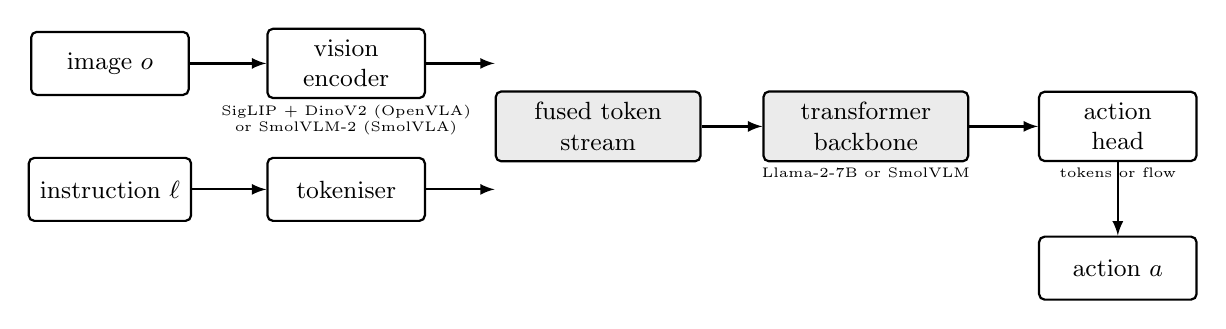
\begin{tikzpicture}[
    every node/.style={font=\small, align=center},
    block/.style={rectangle, draw=black, thick, rounded corners=2pt,
                  minimum width=2.0cm, minimum height=0.8cm, inner sep=4pt},
    fused/.style={rectangle, draw=black, thick, rounded corners=2pt,
                  minimum width=2.6cm, minimum height=0.8cm, inner sep=4pt, fill=black!8},
    arr/.style={-latex, thick},
]
    \node[block] (img) at (0, 2.4) {image $o$};
    \node[block] (lang) at (0, 0.8) {instruction $\ell$};
    \node[block] (visenc) at (3.0, 2.4) {vision\\ encoder};
    \node[block] (tok) at (3.0, 0.8) {tokeniser};
    \node[fused] (fuse) at (6.2, 1.6) {fused token\\ stream};
    \node[fused] (back) at (9.6, 1.6) {transformer\\ backbone};
    \node[block] (head) at (12.8, 1.6) {action\\ head};
    \node[block] (act) at (12.8, -0.2) {action $a$};
    \draw[arr] (img.east) -- (visenc.west);
    \draw[arr] (lang.east) -- (tok.west);
    \draw[arr] (visenc.east) -- (fuse.west |- visenc.east);
    \draw[arr] (tok.east) -- (fuse.west |- tok.east);
    \draw[arr] (fuse.east) -- (back.west);
    \draw[arr] (back.east) -- (head.west);
    \draw[arr] (head.south) -- (act.north);
    \node[font=\tiny, anchor=north] at (3.0, 2.0) {SigLIP $+$ DinoV2 (OpenVLA)\\ or SmolVLM-2 (SmolVLA)};
    \node[font=\tiny, anchor=north] at (9.6, 1.2) {Llama-2-7B or SmolVLM};
    \node[font=\tiny, anchor=north] at (12.8, 1.2) {tokens or flow};
\end{tikzpicture}
\caption{The shared skeleton of OpenVLA and SmolVLA. Image and instruction enter on the left, are encoded into tokens, fused into a single sequence, and passed through a transformer backbone. The action head on the right is the only component that changes shape across the two models: OpenVLA emits discretised action tokens through its language head, SmolVLA emits continuous actions through a flow-matching head.}
\label{fig:vla_skeleton}
\end{figure}

\newthought{Open weights, single-GPU fine-tuning.} The release that makes OpenVLA pedagogically useful is not the architecture but the licence and the recipe. Weights are on the Hugging Face Hub. The reference fine-tuning script supports LoRA, which means a single A100 with eighty gigabytes of memory is enough to adapt the seven-billion-parameter model to a new robot or a new task without rewriting the optimiser. A typical launch looks like this:

\begin{verbatim}
python vla-scripts/finetune.py \
    --vla_path openvla/openvla-7b \
    --data_root_dir /datasets/rlds/ \
    --dataset_name aloha_cube_transfer \
    --run_root_dir /runs/openvla-aloha \
    --adapter_tmp_dir /runs/openvla-aloha/adapters \
    --lora_rank 32 \
    --batch_size 16 \
    --grad_accumulation_steps 1 \
    --learning_rate 5e-4 \
    --image_aug True \
    --wandb_project openvla-ft \
    --save_steps 5000
\end{verbatim}

The command reads a dataset in the RLDS (Reinforcement Learning Datasets) format that Open X-Embodiment standardises on, attaches LoRA adapters to the Llama backbone with rank thirty-two, and trains for as long as the user keeps the job alive. The dataset name is the only argument that ties the run to a specific robot; everything else is generic. After fine-tuning, the adapter weights are a few hundred megabytes, not gigabytes, and they are merged back into the base model only if the user wants a single deployable checkpoint.

\newthought{Inference is even smaller.} Once weights are on disk, running OpenVLA looks much like running any Hugging Face vision-language model, with the small twist that the generated tokens are unbinned into a continuous action vector before being shipped to the controller:

\begin{verbatim}
from transformers import AutoModelForVision2Seq, AutoProcessor
from PIL import Image
import torch

processor = AutoProcessor.from_pretrained(
    "openvla/openvla-7b", trust_remote_code=True)
model = AutoModelForVision2Seq.from_pretrained(
    "openvla/openvla-7b",
    torch_dtype=torch.bfloat16,
    trust_remote_code=True).to("cuda")

image = Image.open("camera_frame.png")
instruction = "pick up the red block and place it on the blue plate"
prompt = f"In: What action should the robot take to {instruction}?\nOut:"

inputs = processor(prompt, image).to("cuda", dtype=torch.bfloat16)
action = model.predict_action(
    **inputs, unnorm_key="bridge_orig", do_sample=False)
% action is a 7-vector: dx, dy, dz, droll, dpitch, dyaw, gripper
robot.step(action)
\end{verbatim}

The salient line is \verb|model.predict_action|, which wraps the autoregressive generation of seven action tokens, the unbinning that turns those tokens back into floats, and the dataset-specific normalisation that scales the floats into the units the controller expects. The same model, with a different \verb|unnorm_key|, drives a different robot. The architecture is universal; the unnormalisation is the embodiment adapter.

\newthought{What each component contributes} can now be stated cleanly. The vision encoder gives the model geometric scene grounding, the ability to perceive that the red cube is to the left of the blue plate and that the gripper is currently above and behind both. The language backbone gives compositional instruction following, the ability to parse novel combinations of verbs and objects that did not appear together in the training trajectories. The action head gives the embodiment-specific output, the ability to translate a high-level intent into the seven floats that this particular arm understands this particular millisecond. Removing any of the three breaks the model in a recognisable and predictable way; OpenVLA's architecture choices are best read as the minimal stack that keeps all three present.

\vspace{2.5em}

\newthought{SmolVLA} sits at the opposite end of the size axis~\cite{Shukor2025SmolVLA}. With roughly four hundred and fifty million parameters, it is fifteen times smaller than OpenVLA, which puts it within reach of a consumer GPU, an Apple Silicon laptop, or a single Jetson Orin running on a robot's onboard compute. The model was released as part of the Hugging Face LeRobot ecosystem and was trained on a mixture of community-collected LeRobot teleoperation data and a curated subset of Open X-Embodiment, deliberately weighted toward small, low-cost arms (the SO-100, the Koch arm, and similar) so that the model is not over-fit to research-lab Frankas.

\marginnote{\newthought{Flow matching, briefly.} A flow-matching head learns a velocity field $v_\theta(a_t, t \mid h)$ conditioned on the backbone's hidden state $h$. To sample, integrate from $a_0 \sim \mathcal{N}(0, I)$ to $a_1$ along $v_\theta$. No discretisation, no vocabulary expansion, smooth continuous actions by construction.}

\newthought{The vision-language backbone} is SmolVLM-2, an open small-scale vision-language model in the same family as the Idefics line. It is not the SigLIP-plus-DinoV2 fusion of OpenVLA; it is a single, smaller, jointly trained vision-language stack. The trade is straightforward: less geometric prior, less semantic capacity, but a backbone whose forward pass fits in a few gigabytes of memory and whose latency is tens of milliseconds rather than hundreds.

\newthought{The action head is the interesting structural difference.} Rather than discretising actions and emitting them through a vocabulary, SmolVLA uses a flow-matching head that produces continuous actions directly. The backbone's hidden state conditions a small velocity-field network; sampling an action is integrating a learned ordinary differential equation from a Gaussian sample to an action vector over a handful of steps. The advantage is that the action is continuous by construction, with no quantisation noise floor, and the head can naturally output multi-step action chunks (a short sequence of actions, say sixteen steps ahead) in one shot rather than one step at a time. The cost is a more complex sampling procedure and a head that has to be trained with a flow-matching objective rather than a cross-entropy.

\newthought{Pedagogical importance.} For students, SmolVLA is the model you can actually run during the practical session. The LeRobot library exposes it through the same training and inference command-line interface as every other policy in the ecosystem. A typical fine-tuning launch reads:

\begin{verbatim}
python lerobot/scripts/train.py \
    --policy.path=lerobot/smolvla_base \
    --policy.device=cuda \
    --dataset.repo_id=lerobot/svla_so100_pickplace \
    --batch_size=64 \
    --steps=20000 \
    --output_dir=outputs/smolvla_so100_ft \
    --job_name=smolvla_pickplace \
    --wandb.enable=true
\end{verbatim}

The dataset \verb|repo_id| points at a Hugging Face dataset of teleoperation episodes recorded on an SO-100 arm; the policy is loaded from the public SmolVLA base checkpoint; the run trains for twenty thousand steps and writes a checkpoint that LeRobot's inference scripts can pick up directly. A laptop with a recent discrete GPU can complete this run in a few hours; a Jetson can do inference in real time on the resulting checkpoint without quantisation.

\newthought{Inference looks the same in shape}, with a different module path and a flow-matching sampling step under the hood:

\begin{verbatim}
from lerobot.common.policies.smolvla.modeling_smolvla \
    import SmolVLAPolicy

policy = SmolVLAPolicy.from_pretrained(
    "outputs/smolvla_so100_ft/checkpoints/last")
policy.to("cuda").eval()

obs = robot.capture()
obs["task"] = "place the cup on the saucer"
with torch.no_grad():
    action_chunk = policy.select_action(obs)
robot.execute(action_chunk)
\end{verbatim}

The key difference visible at the API surface is \verb|select_action| returning an action chunk rather than a single action, reflecting the flow-matching head's natural output shape. Everything else, the observation dictionary, the task string, the policy interface, follows the LeRobot convention shared with the smaller behaviour-cloning baselines that students likely encountered earlier in the course.

\vspace{2.5em}

\newthought{The shared skeleton} is now visible at a glance, and Figure~\ref{fig:vla_skeleton} draws it. Both OpenVLA and SmolVLA encode an image and a language instruction into a fused token stream. Both pass that stream through a transformer backbone whose role is to mix vision, language, and (optionally) proprioceptive state into a hidden representation that is conditional on the entire context. Both end with an action head that turns the hidden representation into a vector the robot can execute. The differences are exactly two: the scale of the backbone, seven billion parameters versus four hundred and fifty million, and the choice of action head, discretised vocabulary tokens versus continuous flow matching.

\newthought{The action-head choice is not cosmetic.} Discretisation buys exactly one thing, the ability to reuse the language backbone's softmax head with no architectural surgery, and pays for it with quantisation error and an awkward separation between the autoregressive action loop and the smooth dynamics of the underlying robot. Flow matching buys continuous, multi-step action chunks at the price of a separate head with its own training objective. Section~3 of this chapter returns to the action-head question as the central frontier debate, because the design axis it opens (do you want actions to live inside the language vocabulary, or outside it as a separate continuous module?) is the axis along which the next generation of VLAs is currently being negotiated.

\vspace{1.5em}

\newthought{What this section sets up.} Concrete VLAs exist, they are open, and they are fine-tunable on hardware students already have access to. OpenVLA shows what a serious seven-billion-parameter manipulation policy looks like when one is willing to pay the compute. SmolVLA shows how far the same architectural recipe can be compressed before the wheels fall off, and where the design choices have to change (the action head, in particular) to make that compression work. The remaining sections of this chapter answer the questions these two models leave open. Section~2 asks what scaffold (data pipeline, simulator, sim-to-real bridge) makes a model like this work in the real world rather than just on the benchmark. Section~3 asks what the frontier (the $\pi_0$ family, RT-2 successors, diffusion-based action heads) adds on top of the OpenVLA-and-SmolVLA baseline~\cite{Brohan2023RT2,Brohan2022RT1,Driess2023PaLME}. Section~4 asks the deepest question: what happens to the action abstraction itself when the same model is allowed to decide whether to move a robot arm or call a function in a software API.


%───────────────────────────────────────────────────────────────────────
% §2  Sim-to-Real, Dexterous Manipulation, and Physics Priors
%───────────────────────────────────────────────────────────────────────

\section{Sim-to-Real, Dexterous Manipulation, and Physics Priors}\index{sim-to-real}\index{equivariance}\index{physics-informed}

\marginnote{\newthought{A side note that earns its keep.} Section~1 named the concrete VLA models. Before we sprint to the frontier in Section~3, we owe a page to the engineering scaffold that makes any of this work in the real world.}

\newthought{Real robot data is precious.} The Open X-Embodiment effort~\cite{Padalkar2024OpenXEmbodiment} aggregated roughly one million trajectories across twenty-two embodiments, the largest cross-lab corpus we have. That is heroic, and it is also roughly six orders of magnitude smaller than the text corpora that train modern language models. Simulation is the obvious escape valve, since simulated rollouts are essentially free. The catch is that a policy trained in simulation almost never transfers to real hardware on its own; the gap between simulator and reality, the so-called sim-to-real gap, is wide enough to make a flawless simulated controller flail on a physical arm. This section walks through the scaffold around VLA training that closes that gap: domain randomisation, the simulators that matter, a brief detour through dexterous manipulation, and the physics priors that turn data efficiency into a structural property of the architecture rather than a property of the dataset.

\vspace{1.5em}

\newthought{Domain Randomisation} attacks the sim-to-real gap by refusing to commit to any single simulator configuration. Vary the lighting, the textures, the friction coefficients, the link masses, the control latency, and the sensor noise across episodes, and the policy is forced to learn an invariance rather than overfit any one set of physics constants~\cite{Tobin2017DomainRandomization}. The real world then becomes one more sample from the randomisation distribution, indistinguishable in principle from any other sampled configuration. The bet is that if the spread of simulated worlds is wide enough, reality lies somewhere inside it, and the policy generalises by accident on purpose.

\newthought{A typical randomisation config} reads like a parameter sheet for a stage play, where every prop has a tolerance:

\begin{verbatim}
domain_randomization:
  visual:
    light_intensity:   [0.4, 1.6]
    light_direction:   uniform_on_sphere
    table_texture:     sample_from(textures/wood, textures/metal, ...)
    camera_pose_jitter:
      position_std_m:   0.02
      rotation_std_deg: 1.5
  dynamics:
    friction:          [0.5, 1.5]
    link_mass_scale:   [0.8, 1.2]
    joint_damping:     [0.7, 1.3]
    actuator_gain:     [0.9, 1.1]
  control:
    action_latency_ms: [0, 40]
    obs_noise_std:     0.01
\end{verbatim}

The exact ranges are domain-specific; the structure is universal. A randomisation block always covers visuals (so the perception head does not memorise pixel statistics), dynamics (so the controller does not memorise inertia), and control (so the policy does not memorise a perfectly synchronised actuator).

\vspace{1.5em}

\newthought{The Simulators that Matter} sit at three corners of the design space. MuJoCo~\cite{Todorov2012MuJoCo} is the de facto standard for contact-rich rigid-body manipulation; its solver handles soft and hard contacts numerically well, which is precisely the regime that breaks naive simulators. Isaac Gym and its successor Isaac Lab~\cite{Makoviychuk2021IsaacGym} push the throughput axis instead: by running the physics step natively on the GPU, a single accelerator simulates roughly sixteen thousand environments in parallel. Training runs that took weeks on real hardware compress into hours of GPU rollouts, and the parallelism is what makes deep reinforcement learning tractable for whole-body locomotion and dexterous control. Open X-Embodiment~\cite{Padalkar2024OpenXEmbodiment} is not a simulator at all; it is the cross-lab dataset that pools real-robot trajectories across embodiments, providing the small but irreplaceable real-world anchor that simulation alone cannot supply. The pragmatic stack uses all three: pretrain in Isaac at massive scale, fine-tune in MuJoCo where contact realism matters, and validate on Open X-Embodiment trajectories before touching hardware.

\begin{table*}[ht]
\centering
\begin{tabular}{p{0.20\textwidth}p{0.22\textwidth}p{0.18\textwidth}p{0.28\textwidth}}
    \toprule
    \textbf{Tool} & \textbf{Strength} & \textbf{Throughput} & \textbf{Typical use} \\
    \midrule
    MuJoCo & contact accuracy & $\sim$1 env on CPU & manipulation research, fine-tuning \\
    Isaac Gym / Lab & GPU parallelism & $\sim$16k envs per GPU & locomotion, large-scale RL \\
    Open X-Embodiment & real-robot trajectories & not a simulator & cross-embodiment finetune and eval \\
    \bottomrule
\end{tabular}
\vspace{2em}
\caption{The three pillars of the modern VLA training stack. Throughput numbers are order-of-magnitude figures and depend strongly on the specific scene complexity.}
\label{tab:vla_simulators}
\end{table*}

\vspace{1.5em}

\newthought{Dexterous Manipulation as a Side Note.} Why dexterous, multi-finger, contact-rich, in-hand manipulation is hard, in five quick beats. The action space is high-dimensional, often twenty or more joints across two hands. The contact state is only partially observable, since tactile sensors are noisy and visual occlusion is the rule rather than the exception. The contact dynamics are fast, with stick-slip transitions that the controller must respond to within milliseconds. Compliance matters more than position accuracy, because rigidly tracking a target trajectory through contact is precisely how things break. And small errors compound through friction, so a millimetre of slip at the fingertip becomes a centimetre of pose error two seconds later. ALOHA-style bimanual setups and the LeRobot software stack have made dexterous benchmarks reproducible enough that cross-lab comparisons are meaningful, and unsurprisingly these are exactly the benchmarks where the sim-to-real gap is most visible. We flag the topic here and move on; dexterity is a research programme of its own, not a paragraph.

\vspace{2.5em}

\newthought{Physics Priors and Geometric Action Spaces} are where this side note earns its pedagogical weight. The argument has five parts.

\newthought{Why pure data-driven policies waste data.} The action space for manipulation is not an abstract vector space; it is the Lie group $\mathrm{SE}(3)$ of rigid-body poses, with rotational substructure $\mathrm{SO}(3)$. A policy that ignores this structure must rediscover from data that picking up a mug is the same task as picking up that same mug after the mug has been rotated by thirty degrees. Each rotated demonstration teaches the policy something it should already know from geometry alone, and each rotation it has not seen at training time is a potential failure case at test time. In a regime where every demonstration is hand-collected on a real robot, paying for geometric facts in trajectories is an expensive way to learn what a single equation could state once.

\newthought{Group-equivariant networks} formalise the right inductive bias~\cite{CohenWelling2016GroupEquivariant}. A network $f$ is equivariant under a group $G$ if, for every group element $g \in G$,
\begin{align*}
    f(g \cdot x) &= g \cdot f(x).
\end{align*}
Read this as a commutativity statement: transforming the input and then applying the network produces the same result as applying the network first and then transforming the output. For $G = \mathrm{SE}(3)$, rotating and translating the scene rotates and translates the predicted action correspondingly, automatically, with no further training. The practical implementations come in two flavours, steerable convolutions that lift the standard convolutional kernel into a representation of the group, and equivariant Transformers that constrain the attention mechanism to respect the same symmetry. Both routes lead to the same place; the architecture, not the dataset, carries the geometric prior.

\newthought{SE(3)-equivariant policies for manipulation} cash this in directly. Neural Descriptor Fields~\cite{Simeonov2022NDF} are the canonical example: a single demonstration of grasping a mug generalises across the full orbit of $\mathrm{SE}(3)$, that is, every rotated and translated configuration of the same mug, for free. A non-equivariant policy needs a demonstration per orbit element, modulo whatever generalisation the network manages on its own. The gain compounds with data scarcity, so the lower the demonstration budget, the larger the relative win from equivariance. Robotics lives permanently in the low-data regime, which is exactly why this inductive bias keeps showing up under different names across the manipulation literature.

\newthought{Soft physics priors via PINNs} are the second flavour of inductive bias. The world-models lecture (Chapter~13) introduced physics-informed neural networks~\cite{Raissi2019PINN} as a way to constrain a learned dynamics model with a residual loss derived from known equations of motion. The same idea constrains policies rather than dynamics: penalise predicted actions that would drive the gripper into static geometry, or that would violate a non-penetration constraint on contact forces, by adding a residual term to the policy loss. Equivariance is a hard prior baked into the architecture; PINN-style residuals are a soft prior baked into the loss. The two are complementary; the choice between them is a choice about how much of your physical knowledge is exact (use a hard prior) and how much is approximate (use a soft prior with a tunable weight).

\newthought{The pedagogical punchline.} The action space of manipulation is geometric. If your policy is not, you are paying for the missing geometry in trajectories, and trajectories are the resource that does not scale. Equivariance is to manipulation what convolution was to vision: the right inductive bias closes orders of magnitude in sample complexity, and once you have it, the rest of the architecture can be ordinary. This is the reason robotics research keeps reinventing equivariance under different names, from spatial transformer networks through neural descriptor fields to whatever the next acronym will be. The names rotate; the underlying claim does not.

\begin{marginfigure}
\begin{tikzpicture}[
    every node/.style={font=\small, align=center},
    block/.style={rectangle, draw=black, thick, rounded corners=2pt,
                  minimum width=1.8cm, minimum height=0.6cm, inner sep=3pt},
]
    \node[block] (x) {scene $x$};
    \node[block, below=14pt of x] (gx) {$g \cdot x$};
    \node[block, right=22pt of x] (fx) {action $f(x)$};
    \node[block, below=14pt of fx] (fgx) {$g \cdot f(x)$};
    \draw[-latex, thick] (x) -- node[above, font=\tiny] {$f$} (fx);
    \draw[-latex, thick] (gx) -- node[below, font=\tiny] {$f$} (fgx);
    \draw[-latex, thick, dashed] (x) -- node[left, font=\tiny] {$g$} (gx);
    \draw[-latex, thick, dashed] (fx) -- node[right, font=\tiny] {$g$} (fgx);
\end{tikzpicture}
\caption{Equivariance as a commuting square. Apply the group action then the policy, or the policy then the group action; the answers agree.}
\label{fig:equivariance_square}
\end{marginfigure}

\vspace{1.5em}

\newthought{Bridging into Section~3.} Section~1 named the concrete VLA models that ship today; Section~2 named the engineering scaffold of simulation, randomisation, and equivariance that makes any of them practical at all. The frontier in Section~3 is what happens when the action head becomes a flow model rather than a discretised classifier, when chain-of-thought reasoning emits actions rather than text, and when one model controls many embodiments at once. The scaffold described here does not vanish at the frontier; it is what the frontier stands on.


%───────────────────────────────────────────────────────────────────────
% §3  Vision-Language-Action as Frontier
%───────────────────────────────────────────────────────────────────────

\section{Vision-Language-Action as Frontier}\index{VLA}\index{cross-embodiment}\index{flow matching}

\marginnote{\newthought{Where Section~3 sits.} Section~1 introduced two open VLAs (OpenVLA and SmolVLA); Section~2 named the engineering scaffold around them, simulation, dexterous manipulation, and physics priors. This section walks the three frontier axes that organise current research and closes on the question students will leave the course with.}

\newthought{The frontier question is not} whether vision-language-action models work; the previous two sections answered that with citations and benchmarks. The frontier question is what shape the action head should take, what scope the model should cover, and what the ceiling looks like for scaling alone. Three axes organise the answers: cross-embodiment generalisation, the design of the action head itself, and the open question of whether the recipe that produced GPT-class language models can carry over to robots when the data does not fit on the internet. The rest of this section walks those axes in order, and ends on the honest question.

\vspace{1.5em}

\newthought{Cross-Embodiment Generalisation.} The first axis answers a question robotics had treated as a punchline for a decade. Single-robot policies do not transfer; every new arm, every new gripper, every new base seems to demand its own dataset and its own training run. Open X-Embodiment~\cite{Padalkar2024OpenXEmbodiment} disproved the assumption at scale: a single transformer trained on roughly one million trajectories pooled from twenty-two distinct robots outperformed each platform's specialist on its own benchmark. The result was not a marginal gain; it was the kind of cross-platform lift that, in vision, only happened once ImageNet pretraining became standard.

\marginnote{\newthought{Why pooling works.} Action spaces look different across embodiments (joint angles for one arm, end-effector deltas for another, base velocities for a mobile platform), but the mapping from (image, instruction) to ``useful next motion'' shares deep structure. Pooling lets the backbone learn that shared structure once and pay for the per-embodiment differences with a small head.}

\newthought{Octo}~\cite{Octo2024GeneralistPolicy} generalised the recipe into a clean template. A generalist transformer policy ingests image and language tokens, produces a latent that encodes the task, and a lightweight action head per embodiment decodes the latent into the platform's native control space. The same backbone serves a Franka arm, a WidowX, and a mobile manipulator; only the small head changes. The structural lesson of cross-embodiment training is the inverse of the lesson everyone expected. The bottleneck of robotic learning is not policy capacity. It is data scarcity per embodiment, and pooling across embodiments amortises the cost of every single trajectory across every single robot the pool contains.

\newthought{The implication for engineering practice} is that the right question to ask of a new robot is no longer ``what is its dataset?''. It is ``what tokeniser does its action space need, and which existing pool does its observation space resemble?''. A new arm with a parallel gripper inherits most of its policy from the existing pool; the marginal cost of supporting it is a few thousand demonstrations and a fresh head, not a fresh model. Section~4 will pick up this thread when it argues that orchestration patterns, not bigger backbones, are the next compounding lever.

\vspace{2.5em}

\newthought{Action Heads: Discrete Tokens vs Continuous Flow Matching.} The second axis is where the field has split into two camps, and where the most consequential design choice in any VLA actually lives. Both camps share the same backbone story, a vision-language model pretrained on web data and fine-tuned on robot trajectories. They disagree on the last layer. One camp emits discrete action tokens through the same softmax that emits text. The other camp pipes the backbone's latent into a separate continuous head that samples trajectories with flow matching. The choice determines what the model can do, how fast it runs, and how cleanly it composes with the rest of a robot stack.

\newthought{Discrete action tokens, the RT-2 family.} Bin each action dimension into a fixed alphabet (RT-2 uses 256 bins per dimension)~\cite{Brohan2023RT2}, reserve a stretch of the language model's vocabulary for those bins, and let the autoregressive softmax that emits ``the cat sat on the mat'' emit ``\texttt{<act\_bin\_117> <act\_bin\_204> ...}'' instead. OpenVLA~\cite{Kim2024OpenVLA} adopts the same approach with an open backbone and the Open X-Embodiment training mix. The advantages are real and pedagogically clean. The language model's reasoning machinery is fully available, because actions look like words. Chain-of-thought can interleave with action emission without any architectural change. One tokeniser handles every embodiment in the pool, because the bins live in a shared vocabulary that the backbone already knows how to produce.

\marginnote{\newthought{The tokeniser is the trick.} The bins are not learned; they are a fixed quantisation of the action range. The policy never has to learn that ``$0.03$ metres in $x$'' means anything; it only has to learn which bin id to emit next, which is the same thing the language model has been doing for trillions of tokens of text.}

\newthought{The disadvantages are equally real.} Quantisation injects a floor of error that does not go away with more compute; finer bins help, but the autoregressive cost grows. Decoding is slow at high control rates because each action dimension is a forward pass; emitting a six-dimensional end-effector delta at 50 Hz means three hundred token forward passes per second per robot. Smoothness across timesteps is not built into the head; the model must learn from data that consecutive actions should not jitter, a property that a continuous-output head gets for free.

\newthought{Continuous flow matching, the $\pi_0$ approach.} The other camp keeps the backbone but replaces the discrete head with a flow-matching network that samples continuous action trajectories conditioned on the backbone's latent. The $\pi_0$ model~\cite{Black2024Pi0} pioneered the recipe at scale: a vision-language backbone produces a task-conditioned latent, and a flow-matching action expert (trained with the same loss family that drives modern image and video generation) integrates a learned vector field from noise to a smooth action trajectory in continuous space. The output is not a single action; it is a short chunk of continuous trajectory, sampled in a handful of integration steps.

\marginnote{\newthought{Flow matching in one line.} Train a vector field $v_\theta(a, t \mid \text{ctx})$ to push samples along a path from noise at $t{=}0$ to data at $t{=}1$, conditioned on the backbone's context vector. At inference, integrate the field for a few Euler steps. The action arrives as a continuous vector, not a string of bin ids.}

\newthought{The advantages are control-theoretic.} The output lives in the action space the robot actually consumes, with no quantisation floor. Multimodal action distributions, two equally valid ways of grasping the same mug, are handled natively, because the flow head learns a distribution rather than a single mode. Fine motor control such as in-hand reorientation and contact-rich insertion benefits from the smoother, faster trajectories. The disadvantages are conceptual. The action head is a separate model with its own training loss; the unified ``one model, one tokeniser'' story breaks. Chain-of-thought interleaving becomes harder, because the model cannot easily explain itself between sampling steps of a flow integrator.

\begin{table*}[ht]
\centering
\begin{tabular}{p{0.20\textwidth}p{0.34\textwidth}p{0.34\textwidth}}
    \toprule
    \textbf{Property} & \textbf{Discrete tokens (RT-2, OpenVLA)} & \textbf{Continuous flow ($\pi_0$)} \\
    \midrule
    Output space & quantised bin ids in language vocabulary & continuous trajectory chunks in native action space \\
    Decoding & autoregressive softmax, one pass per dimension & few-step integration of a learned vector field \\
    Smoothness & must be learned from data & built into the integrator \\
    Multimodality & captured only via temperature, often collapses to mode & native, the flow learns the distribution \\
    Chain-of-thought & interleaves naturally with actions & harder, the head is a separate model \\
    Cross-embodiment tokeniser & one shared vocabulary across robots & one shared latent, per-embodiment flow head \\
    Throughput at high control rates & limited by autoregressive cost & higher, integration is parallel across the chunk \\
    \bottomrule
\end{tabular}
\vspace{2em}
\caption{Two action-head philosophies. Discrete tokens push the policy toward language modelling; continuous flow pulls it toward control theory. Each row is a real engineering trade, not a marketing distinction.}
\label{tab:action_heads}
\end{table*}

\newthought{Reading the difference in pseudocode} makes the gap concrete. Both excerpts assume the backbone has already produced a context vector \texttt{ctx} from the image and the instruction; only the head differs.

\begin{verbatim}
% Discrete-token decoding (RT-2 / OpenVLA style).
ctx = backbone(image, instruction)
action = []
for dim in range(action_dim):
    logits = lm_head(ctx, history=action)
    bin_id = sample(softmax(logits))
    action.append(dequantize(bin_id, dim))

% Continuous flow-matching decoding (pi-zero style).
ctx = backbone(image, instruction)
a    = sample_noise(shape=(horizon, action_dim))
for t in linspace(0.0, 1.0, num_steps):
    a = a + dt * flow_head(a, t, ctx)
trajectory = a
\end{verbatim}

\newthought{The pseudocode shows the asymmetry plainly.} The token path runs a loop over action dimensions and stays inside the language model. The flow path runs a loop over integration time and lives in a separate module. Both produce an action; the question is which loop you would rather pay for at deployment, and which loop composes more naturally with the rest of your stack.

\begin{figure}
\centering
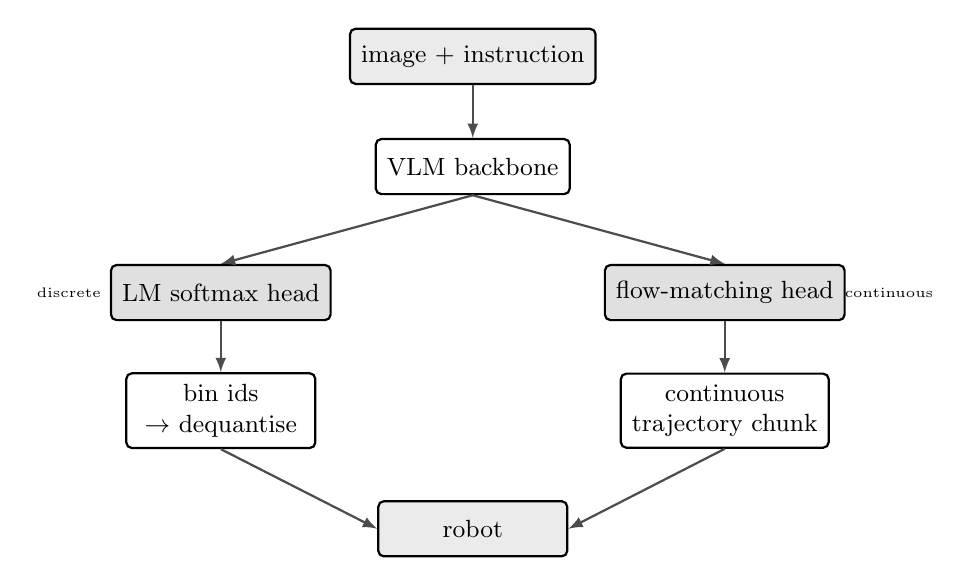
\begin{tikzpicture}[
    every node/.style={font=\small, align=center},
    block/.style={rectangle, draw=black, thick, rounded corners=2pt,
                  minimum width=2.4cm, minimum height=0.7cm, inner sep=4pt},
    arr/.style={-latex, thick, black!70},
]
    \node[block, fill=black!8] (img) at (0, 3.0) {image $+$ instruction};
    \node[block] (back) at (0, 1.6) {VLM backbone};
    \draw[arr] (img.south) -- (back.north);
    \node[block, fill=black!12] (lm) at (-3.2, 0.0) {LM softmax head};
    \node[block] (bins) at (-3.2, -1.5) {bin ids \\ $\to$ dequantise};
    \draw[arr] (back.south) -- (lm.north);
    \draw[arr] (lm.south) -- (bins.north);
    \node[font=\tiny, anchor=east] at (-4.6, 0.0) {discrete};
    \node[block, fill=black!12] (flow) at (3.2, 0.0) {flow-matching head};
    \node[block] (traj) at (3.2, -1.5) {continuous \\ trajectory chunk};
    \draw[arr] (back.south) -- (flow.north);
    \draw[arr] (flow.south) -- (traj.north);
    \node[font=\tiny, anchor=west] at (4.6, 0.0) {continuous};
    \node[block, fill=black!8] (robot) at (0, -3.0) {robot};
    \draw[arr] (bins.south) -- (robot.west);
    \draw[arr] (traj.south) -- (robot.east);
\end{tikzpicture}
\caption{Two action-head architectures sharing the same backbone. The left branch emits discrete bin ids through the language model's softmax; the right branch emits continuous trajectory chunks through a flow-matching head. The split happens at the backbone's output, not earlier.}
\label{fig:action_heads}
\end{figure}

\newthought{The structural insight that closes this axis.} The choice of action head is the choice of how much the policy borrows from language modelling. Discrete tokens push the policy toward the language model; the action becomes another kind of word, and the price is quantisation and slower decoding. Continuous flow pulls the policy toward control theory; the action becomes a sample from a learned distribution over trajectories, and the price is a separate module that does not chain-of-thought as naturally. The frontier today is split between these camps and is likely to converge on hybrids in which the language model emits a high-level plan token (``move to the bowl, then drop'') and a flow head emits the fine-grained continuous motion. Section~4 will argue that this is the orchestration pattern of agentic systems instantiated inside a single robot policy.

\vspace{2.5em}

\newthought{Chain-of-Thought That Emits Actions.} RT-2's signature feature is the unification of two behaviours that, before it, lived in different systems. The model can reason in natural language, ``the apple is to the left of the bowl, so I need to move my gripper roughly fifteen centimetres to the right and then close,'' and then emit a discretised action token as the next token in the same stream. The chain-of-thought machinery that solves a maths word problem is the same machinery that decomposes a manipulation task; only the final tokens are interpreted as motor commands rather than as text. Nothing about the architecture changes between the reasoning and the acting; only the consumer of the output tokens differs.

\marginnote{\newthought{Why this matters more than it seems.} The unification means that any improvement to the backbone's reasoning, longer context, better instruction following, sharper spatial grounding, transfers directly to the policy. The robot inherits the language model's progress for free, because it is the language model.}

\newthought{The conceptual unification} is the bridge that Section~4 makes explicit. Actions are tokens; tokens are actions. An action token that says ``close the gripper'' is, structurally, the same object as a tool-use token that says ``call the calendar API''. Both are emitted by the same softmax; both are interpreted by an external system. The robot is one such external system; an HTTP client is another. The chain-of-thought that solves a multi-step manipulation task is the chain-of-thought that solves a multi-step booking task. Section~4 builds this argument out; the point here is that the unification is already present inside RT-2 and is what makes the next axis possible.

\vspace{2.5em}

\newthought{Frontier Exemplars.} Two proprietary systems represent the current state of practice and are worth knowing about even though their code and weights are not open. They illustrate, respectively, the orchestration pattern that Section~4 will formalise and the bet that frontier model labs are placing on VLA-as-Gemini rather than on a specialised robotics stack.

\newthought{Helix, from Figure AI}~\cite{FigureAI2025Helix}, ships a dual-system architecture on a humanoid robot. A fast low-level controller runs at roughly 200 Hz and produces continuous joint commands; a slower vision-language reasoner runs at roughly 8 Hz and produces high-level goals and constraints that the fast controller follows. The two systems share a humanoid body and a common observation stream; they do not share a model. The architectural pattern is the orchestration pattern of Section~4 instantiated in hardware: one model reasons slowly about what to do, another model executes quickly how to do it, and the interface between them is small. The pattern is not unique to Helix; it is the natural answer to the throughput mismatch between language-model inference and motor control, and it generalises far beyond humanoids.

\newthought{Gemini Robotics, from Google DeepMind}~\cite{GeminiRobotics2025}, fine-tunes a Gemini-class vision-language model for robotic action and adds extensions for spatial reasoning, in-context tool use, and dexterous manipulation. The bet underneath the system is significant: rather than build a specialised robotics stack, the team is treating a frontier multimodal model as the substrate, and adding only the minimum machinery needed to ground it in a body. The implicit hypothesis is that the same scaling that produced GPT-class reasoning will, with the right action head and the right data, produce general-purpose physical agents. Whether the hypothesis holds is the subject of the next axis.

\vspace{2.5em}

\newthought{Does Scaling Solve Robotics?} The optimistic view is well supported. Scaling laws hold for cross-embodiment training; Open X-Embodiment showed that more robots, more trajectories, and more parameters keep producing gains, and the curves do not show signs of plateauing within the budgets tried so far. OpenVLA generalises to held-out robots with small fine-tuning sets. The $\pi_0$ model hits in-hand manipulation tasks that single-task baselines simply cannot perform. The evident path forward, if you take the optimistic view, is more data, more compute, and more cross-embodiment fusion, the same recipe that took language models from playthings to infrastructure in roughly a decade.

\newthought{The pessimistic view is grounded in arithmetic.} Robot data is not on the internet. A trajectory requires a physical robot, a physical setup, hardware time, and (almost always) human teleoperation or human supervision. Open X-Embodiment, the largest open pool, sits at roughly $10^6$ trajectories. ImageNet was $1.4 \times 10^7$ labelled images, and image-text web pairs run to $10^9$ or more. Internet text is on the order of $10^{13}$ tokens. Robotics data is roughly six orders of magnitude smaller than language data, and it is growing roughly linearly in the number of robots deployed, not exponentially in the way web text grew. There is no scraping equivalent for trajectories; the data wall is a property of the medium, not of the engineering effort applied to it.

\begin{figure}
\centering
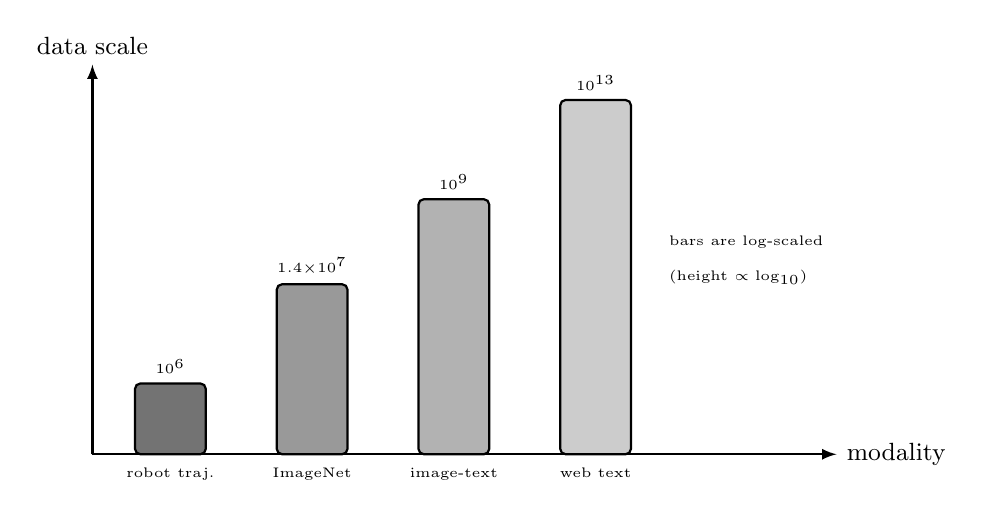
\begin{tikzpicture}[scale=0.9, every node/.style={font=\small}]
    \draw[thick, -latex] (0,0) -- (10.5,0) node[anchor=west, font=\small] {modality};
    \draw[thick, -latex] (0,0) -- (0,5.5) node[anchor=south, font=\small] {data scale};
    \draw[thick, fill=black!55, rounded corners=2pt] (0.6,0) rectangle (1.6,1.0);
    \node[font=\tiny, anchor=south] at (1.1,1.0) {$10^6$};
    \node[font=\tiny, anchor=north] at (1.1,-0.05) {robot traj.};
    \draw[thick, fill=black!40, rounded corners=2pt] (2.6,0) rectangle (3.6,2.4);
    \node[font=\tiny, anchor=south] at (3.1,2.4) {$1.4{\times}10^7$};
    \node[font=\tiny, anchor=north] at (3.1,-0.05) {ImageNet};
    \draw[thick, fill=black!30, rounded corners=2pt] (4.6,0) rectangle (5.6,3.6);
    \node[font=\tiny, anchor=south] at (5.1,3.6) {$10^9$};
    \node[font=\tiny, anchor=north] at (5.1,-0.05) {image-text};
    \draw[thick, fill=black!20, rounded corners=2pt] (6.6,0) rectangle (7.6,5.0);
    \node[font=\tiny, anchor=south] at (7.1,5.0) {$10^{13}$};
    \node[font=\tiny, anchor=north] at (7.1,-0.05) {web text};
    \node[font=\tiny, anchor=west] at (8.0,3.0) {bars are log-scaled};
    \node[font=\tiny, anchor=west] at (8.0,2.5) {(height $\propto \log_{10}$)};
\end{tikzpicture}
\caption{The embodied data wall. Robotic trajectory pools are roughly six orders of magnitude smaller than the corpora that drove the language scaling story, and they grow with deployed hardware rather than with crawls. Bar heights are proportional to $\log_{10}$ of the trajectory or token count.}
\label{fig:data_wall}
\end{figure}

\newthought{The honest answer} is that scaling helps a lot but does not close the gap on its own. The mitigations the field is exploring all attack the data wall from different angles. Cross-embodiment pooling, the lever this section opened with, multiplies the effective dataset by treating every robot's trajectories as training signal for every other robot's policy. Simulation, covered in Section~2, generates trajectories cheaply at the cost of a sim-to-real distribution shift that has to be closed by other means. Self-collected data via deployed fleets, the strategy implicit in any company that sells robots, scales linearly with hardware in the wild, and turns deployment into data acquisition. Pretraining on web-scale video, where billions of frames already exist, can teach affordances and physical intuitions even without action labels, and a vision-language backbone trained on such video is a stronger starting point for any action head. None of these mitigations is a clear winner yet, and most teams use several at once.

\marginnote{\newthought{The frontier is honest.} No one in the field claims to have solved the embodied data problem. The published systems all improve along one or two of the mitigation axes; none has bent the curve. This is the right note for the lecture series to leave open: scaling helps, but scaling alone does not buy general-purpose robotics, and the question of what does is genuinely unresolved.}

\newthought{The open question}, then, is the one students should leave the course holding. Will cross-embodiment pooling, simulation, fleet-collected data, and video pretraining together close the six-order-of-magnitude gap to web text? Or will general-purpose physical intelligence require a fundamentally different recipe than the one that produced general-purpose language? Neither answer is yet supported by the evidence; both are taken seriously by serious people. The course ends, deliberately, with the question still open.

\vspace{2.5em}

\newthought{Bridge into Section~4.} An action token emitted by a chain-of-thought, a continuous trajectory sampled by a flow head, a high-level goal passed from a slow VLM to a fast controller in a Helix-style stack: these are the same object viewed at different temporal resolutions. They are tokens that happen to be actions. Section~4 makes the observation explicit and shows that the same orchestration pattern unifies robotic VLAs with the agentic language models that emit API calls instead of motor torques. The robot calling \texttt{close\_gripper()} and the assistant calling \texttt{book\_calendar()} are the same architecture; only the actuator differs.


%───────────────────────────────────────────────────────────────────────
% §4  Orchestration and Agentic Tool Use
%───────────────────────────────────────────────────────────────────────

\section{Orchestration and Agentic Tool Use}\index{orchestration}\index{agentic AI}\index{tool use}

\marginnote{\newthought{Action is a token sequence.} The action space is the only thing that changes between a robot, a researcher, and a desktop assistant. Once that line is accepted, embodied AI and agentic AI stop being two fields.}

\newthought{The unification beat that closes this chapter} is also the closing beat of the course. Every architecture we have looked at in Sections~1 to~3 has been a policy that maps an observation into a token sequence whose tokens are then read as actions. RT-2 reads its tokens as motor torques, OpenVLA reads them as gripper deltas, PaLM-E reads them as a mixed stream of language and control. The choice of action space is a downstream decision: motor torques, API calls, lines of Python, mouse coordinates, function names, search queries. The architecture does not change. Once we accept this, the wall between embodied AI and agentic AI dissolves; they are the same field viewed through different action spaces, and the rest of this section walks the variants.

\vspace{2.5em}

\newthought{Hierarchical orchestration} is the first variant, and it predates the modern VLA literature by a wide margin. A high-level language model serves as the planner; a low-level policy serves as the executor; the planner decomposes a goal into subtasks and the executor carries each subtask out. The planner thinks in language because language is the substrate it was pretrained on; the executor thinks in motor primitives or tool calls because that is the substrate the world responds to.

\newthought{SayCan}~\cite{Ahn2022SayCan} is the canonical instantiation of the pattern. A large language model proposes candidate next actions in natural language, a learned affordance model scores how feasible each candidate is in the current scene, and the product of language likelihood and affordance score chooses the action. The planner contributes semantic reasonableness; the affordance grounding contributes physical plausibility; neither alone is sufficient. SayCan was the first system to make the case that an off-the-shelf language model could plan robot behaviour without ever having seen a robot, provided the affordance head was kept honest by interaction data.

\newthought{PaLM-E}~\cite{Driess2023PaLME} collapses the two halves into a single backbone. Instead of running a separate planner and a separate affordance scorer, PaLM-E ingests image tokens, state tokens, and language tokens through one transformer and emits an action plan in the same stream. The planner and the executor share parameters; the embedding space is the only place the modalities meet. The hierarchy is logical, not architectural; one network does both jobs and the human-readable plan is just one slice of its output.

\newthought{Helix in Section~3} is the same pattern instantiated in robotic hardware. System~2 reads the scene at a few hertz and emits a latent task description; System~1 takes that latent at two hundred hertz and emits motor torques. The planner is slow, deliberate, language-shaped; the executor is fast, reactive, motor-shaped. The bandwidth gap between them is what makes the decomposition useful: the planner thinks in seconds, the executor acts in milliseconds, and the latent embedding bridges the rates.

\begin{figure}
\centering
\begin{tikzpicture}[
    every node/.style={font=\small, align=center},
    block/.style={rectangle, draw=black, thick, rounded corners=2pt,
                  minimum width=2.4cm, minimum height=0.85cm, inner sep=4pt},
    arr/.style={-latex, thick, black!75},
    fbarr/.style={-latex, thick, black!45, densely dashed},
]
    \node[block, fill=black!8] (goal) {goal $g$\\(language)};
    \node[block, right=18pt of goal] (planner) {planner\\(LM)};
    \node[block, right=18pt of planner] (sub) {subtask\\tokens $s_t$};
    \node[block, right=18pt of sub, fill=black!12] (exec) {executor\\(VLA / tool)};
    \node[block, right=18pt of exec] (env) {environment};
    \draw[arr] (goal.east)    -- (planner.west);
    \draw[arr] (planner.east) -- (sub.west);
    \draw[arr] (sub.east)     -- (exec.west);
    \draw[arr] (exec.east)    -- (env.west);
    \draw[fbarr] (env.south) .. controls +(0,-0.9) and +(0,-0.9) .. (planner.south)
        node[midway, below, font=\tiny, black!55] {observation feedback};
\end{tikzpicture}
\caption{Hierarchical orchestration. A planner consumes a goal and emits subtask tokens which the executor consumes as actions. Observations from the environment loop back to the planner so it can replan when the world surprises it. The planner is slow and language-shaped; the executor is fast and action-shaped.}
\label{fig:orchestration}
\end{figure}

\marginnote{\newthought{Same shape as Mixture-of-Experts.} A small router decides which large specialist gets the next token. Orchestration is MoE on the time axis: the planner is the router, the executor is the expert, and the tokens it routes are subtasks rather than tensor activations.}

\newthought{The orchestration pattern is structurally a Mixture-of-Experts.} A small, fast network decides what a large, slow specialist will be asked to handle next. In MoE the routing happens per token inside one forward pass; in orchestration it happens per subtask across many forward passes; in Helix it happens at the rate gap between Systems~1 and~2. The recurring unit is a small router and a large expert. Once the eye is trained to see it, the pattern shows up everywhere from sparse transformers to surgical robots.

\vspace{2.5em}

\newthought{Agentic tool use as a generalised action space} is the second variant, and it is the place where the unification frame becomes inescapable. If the action space can be motor torques, why not API calls? If it can be API calls, why not lines of Python? If it can be Python, why not mouse coordinates? Every step further along that list keeps the architecture identical and only swaps out the interpretation layer that turns tokens into world effects.

\newthought{ReAct}~\cite{Yao2023ReAct} makes the swap concrete for tool calls. The model alternates between two kinds of tokens: \texttt{Thought:} tokens that carry chain-of-thought reasoning, and \texttt{Action:} tokens that emit a tool invocation. After every \texttt{Action:} the system pauses, runs the tool, splices the tool's response back into the context as an \texttt{Observation:}, and lets the model continue. The reasoning is interleaved with the acting; neither is privileged. The action space is the set of tool calls available to the agent, and the policy is the same autoregressive language model that, in Section~1, would have emitted gripper deltas.

\begin{verbatim}
Question: How tall is the building that houses the
          Anthropic San Francisco office, in metres?

Thought: I need the address first, then the building height.
Action:  search("Anthropic San Francisco office address")
Observation: "Anthropic, One Front Street, San Francisco, CA"

Thought: Now I need the height of One Front Street.
Action:  lookup("One Front Street San Francisco height metres")
Observation: "One Front Street: 700 ft (213 m), 38 floors."

Thought: I have the answer.
Action:  finish("Approximately 213 metres.")
\end{verbatim}

\newthought{The trace looks alien only at first glance.} Replace \texttt{search} with \texttt{move\_arm}, replace \texttt{lookup} with \texttt{open\_gripper}, and the same loop is what an OpenVLA execution log looks like in Section~1. The same chain-of-thought machinery that emits robot actions in RT-2 emits search queries here; the difference is which interpreter is wired up at the back of the model.

\newthought{Toolformer}~\cite{Schick2023Toolformer} pushes the unification one step deeper, into self-supervision. Rather than fine-tuning on human-annotated tool-use traces, Toolformer asks a base language model to propose, for each position in its own training corpus, a candidate tool call that might help predict the next tokens. The system actually executes each candidate; it keeps a tool call only if substituting the tool's response for the surrounding context would have lowered the next-token loss; the surviving calls are interleaved with the original text and the model is trained on this augmented corpus. The agentic capability is bootstrapped without a single human label; the supervision comes from the language model's own predictive distribution disagreeing with reality and a tool's response improving the agreement.

\marginnote{\newthought{Self-supervision, again.} Toolformer's training signal is exactly the perplexity gap that drove masked language modelling and CLIP. The corpus tells the model when a tool would have helped, and the model learns to predict that signal. The same principle that made encoders made tool users.}

\newthought{This is the course's self-supervision thread} arriving at agency. Chapter~9 used pretext tasks to learn representations; Toolformer uses next-token prediction to learn when to reach outside the context window. The objective has not changed; the action space has. The lesson generalises: any time a foundation model can score whether an action would have helped, it can also learn, without a teacher, when to take that action.

\newthought{Code as Policies}~\cite{Liang2023CodeAsPolicies} pushes the action space one further notch. Instead of emitting a single tool call, the model emits a program. The action token sequence is Python (or pseudocode), and the runtime interprets it by calling robot primitives, library functions, or other models as the program dictates. Loops become loops; conditionals become conditionals; recursion becomes recursion. Compositional manipulation, the kind of task that RT-2 struggles with because each step must be predicted in isolation, becomes a control-flow problem the language model already knows how to solve.

\begin{verbatim}
% Goal: sort the objects on the table by colour into the bins.
objects = detect_objects()
bins    = {"red": (0.4, 0.2), "green": (0.4, 0.0), "blue": (0.4, -0.2)}

for obj in objects:
    colour = classify_colour(obj)
    if colour not in bins:
        say(f"No bin for {colour}, skipping.")
        continue
    pick(obj)
    place(obj, bins[colour])

if all(is_empty(region) for region in table_regions()):
    say("Table is sorted.")
\end{verbatim}

\newthought{The verbatim above is a policy.} The action space is the language of Python programs that close over a small library of robot primitives. The policy is the language model that emits the program; the execution is the interpreter that runs it. This is a generalisation of ReAct in the same sense that programs are a generalisation of straight-line traces; the chain-of-thought has been promoted to a control-flow graph.

\vspace{2.5em}

\newthought{Long-horizon agents} are the third variant, and they push the action abstraction across hours and across modalities until the question of what counts as embodiment becomes uncomfortable to answer.

\newthought{Voyager}~\cite{Wang2023Voyager} is the canonical example of an agent that learns by acting. A GPT-4 backbone drives a Minecraft client through a code-as-action interface much like Code as Policies; an automatic curriculum proposes new goals based on what the agent has and has not yet achieved; a skill memory stores every successful program the agent writes so that later programs can call earlier ones as subroutines. The agent is open-ended in the literal sense: there is no fixed task list, the curriculum keeps writing new ones, and the skill library keeps growing. By the end of a long run, Voyager has authored, debugged, and reused dozens of programs that no human supplied. The distinction between training data and test behaviour has dissolved; the agent's history is its training set.

\newthought{SWE-agent}~\cite{Yang2024SWEAgent} drags the same machinery into software engineering. The action space is now: read a file, edit a span of lines, run a shell command, list a directory, search for a symbol, run the test suite. The environment is a repository and a working terminal. The tasks are real GitHub issues, drawn from the SWE-bench evaluation, that require understanding a multi-file codebase well enough to localise a bug and fix it without breaking anything else. Tasks span what a human engineer would think of as hours of work, and the agent solves a respectable fraction of them. The IDE has become the agent's body; the file system is its workspace; the test suite is its proprioception. Embodiment is not gone, it has migrated.

\newthought{Computer-use agents}~\cite{Anthropic2024ComputerUse} are the most general non-physical embodiment shipped to date. The model observes a screenshot of a desktop and emits actions in the space of mouse events, keyboard events, and waits. The action space is, as nearly as makes no difference, the set of things a person can do at a computer. There is no domain-specific tool API to memorise; the agent's interface is the same one a human would use, and any application that can be operated by a human can in principle be operated by the model.

\begin{verbatim}
[t=0.0s] observe_screenshot()
         -> desktop, browser open at https://example.com/login
[t=0.4s] click(x=412, y=288)
[t=0.5s] type("alex@example.com")
[t=1.1s] click(x=412, y=332)
[t=1.2s] type("hunter2")
[t=1.4s] click(x=480, y=388)
[t=2.0s] observe_screenshot()
         -> dashboard, "Welcome, Alex" visible
[t=2.1s] click(x=92, y=160)
[t=3.0s] observe_screenshot()
         -> reports list rendered
[t=3.1s] click(x=240, y=412)
[t=3.4s] observe_screenshot()
         -> file saved to ~/Downloads/q3.pdf
\end{verbatim}

\marginnote{\newthought{The screen is a body.} Mouse coordinates are motor torques on a flat manifold; keystrokes are gripper actions on a discrete one. The action heads are different, the architecture above them is the same.}

\newthought{Read that trace as a robot trajectory} and the unification frame becomes undeniable. Replace screenshots with camera frames, replace clicks with end-effector poses, replace keystrokes with gripper commands, and the log is structurally identical to the OpenVLA log of Section~1. A VLA whose action head emits mouse coordinates is a robot whose body is a screen; a robot whose action head emits motor torques is an agent whose desktop is the physical world.

\vspace{2.5em}

\newthought{The unification frame, re-stated.} Robot action heads emit motor torques. ReAct emits search queries. Code as Policies emits Python. Computer-use agents emit clicks. SWE-agent emits file edits and shell commands. SayCan emits next-action proposals scored by an affordance head. They share one architecture: a language-model-class backbone whose tokens are interpreted, by some downstream layer, as actions in some action space. The VLA paradigm subsumes both robotic control and LLM agents because both are policies over token-action spaces, and the action space is a choice that does not change the architecture above it.

\newthought{What does change with the action space} is the interpreter behind the head, the data the policy is trained on, and the reward signal that shapes it. The transformer in the middle is the same transformer; the embeddings are the same embeddings; the autoregressive loop is the same loop. The lesson the field has internalised over the past three years is that this middle layer is a substrate that works in any action space we have so far cared to wire up to it. Embodiment is not a property of the architecture; it is a property of the interface.


%───────────────────────────────────────────────────────────────────────
% Course-level closing (move to end of Block 3 when assembled)
%───────────────────────────────────────────────────────────────────────

\newthought{The course began with clustering points in $\mathbb{R}^d$,} and it ends with policies that emit tokens which happen to be actions in the world. The thread connecting the two is that pattern emerges from data, and the pattern increasingly looks like what to do next. Unsupervised learning has turned out to be how we taught machines to act, even though almost none of the lectures in this series talked about action until the last few.

\newthought{Trace the arc explicitly.} Acts I and II of the course were geometry: clusters in $\mathbb{R}^d$, then embeddings that bent that geometry to match meaning. Act III was epistemic supervision: zero-shot transfer, self-supervised pretext, learning without labels by exploiting structure already in the data. Act IV was noisy supervision: weak labels, demonstrations, judges, the Snorkel-shaped pipelines that scale annotation past what humans can do alone. The reinforcement learning lecture added reward and made action explicit. The world models lecture added imagination and let the agent rehearse before acting. This last lecture took those threads and let the agent act in any space we are willing to define for it.

\newthought{The course is finished; the field is not.} The seven acts above each took a decade or more to crystallise into the form we taught here, and each rests on assumptions that the next decade will probably revise. The action abstraction is the youngest of them and the most likely to keep moving. What we can say with some confidence is that the substrate is shared; that the unsupervised, self-supervised, and weakly-supervised learning we have spent fourteen chapters on is the part that does not change when the action space does; and that whatever the next embodiment turns out to be, the lectures you have just finished are the part that survives.
